\documentclass{report}
\usepackage{array}
\usepackage{longtable}
\usepackage{textcase}
\usepackage[utf8]{vietnam}
\usepackage{graphicx}
\usepackage{scrextend}
\usepackage[left=3.5cm,right=2cm,top=3.5cm,bottom=3cm]{geometry}
\usepackage{xhfill}
\usepackage{floatrow}
\usepackage{subfigure}
\usepackage{wrapfig}
\usepackage{lipsum}
\usepackage{lettrine}
\usepackage[
    backend=biber,
    style=authoryear,
    natbib=true,
    url=true, 
    doi=true,
    eprint=false
]{biblatex}
\usepackage{hyperref} 
\addbibresource{myref.bib}

\begin{document}
\newcommand{\xfill}[2][1ex]{{%
  \dimen0=#2\advance\dimen0 by #1
  \leaders\hrule height \dimen0 depth -#1\hfill%
}}

%Page 1
\changefontsizes[14pt]{12pt}
\centerline{TỔNG LIÊN ĐOÀN LAO ĐỘNG VIỆT NAM}

\changefontsizes[14pt]{11pt}
\centerline{\textbf{TRƯỜNG ĐẠI HỌC TÔN ĐỨC THẮNG}}
\centerline{\textbf{KHOA CÔNG NGHỆ THÔNG TIN}}

\begin{center}
    \begin{figure}[htp]
    \begin{center}
     
\includegraphics[scale=.2]{logo}
    \end{center}
    \end{figure}
\end{center}

\changefontsizes{16pt}
\centerline{\textbf{BÀI TẬP LỚN: NHẬP MÔN MẠNG MÁY TÍNH}}
\vspace{1.5cm}
\changefontsizes{24pt}
\centerline{\textbf{XÂY DỰNG MẠNG MÁY TÍNH}}
\centerline{\textbf{CHO NHÀ C TRƯỜNG ĐẠI HỌC}}
\centerline{\textbf{TÔN ĐỨC THẮNG}}

\vspace{4cm}
\begin{flushright}
\renewcommand{\baselinestretch}{0.05}
\changefontsizes{14pt}
\textit{Người hướng dẫn: }\textbf{G.V Mai Ngọc Thắng}
\setlength{\parskip}{0.5em}

\textit{Người thực hiện: }\textbf{Trần Quốc Lĩnh - 51703124}
\setlength{\parskip}{0.5em}

\textit{}\textbf{Hà Huy Tường - 51703222}
\setlength{\parskip}{0.5em}

\textit{}\textbf{Phan Đức Anh - 51702058}
\setlength{\parskip}{0.75em}

Khoá: \textbf{21}
\setlength{\parskip}{0.5em}

\end{flushright}

\vspace{1cm}
\changefontsizes{14pt}
\centerline{\textbf{THÀNH PHỐ HỒ CHÍ MINH, NĂM 2018}}


%Page 2
\newpage
\changefontsizes[14pt]{12pt}
\centerline{TỔNG LIÊN ĐOÀN LAO ĐỘNG VIỆT NAM}

\changefontsizes[14pt]{11pt}
\centerline{\textbf{TRƯỜNG ĐẠI HỌC TÔN ĐỨC THẮNG}}
\centerline{\textbf{KHOA CÔNG NGHỆ THÔNG TIN}}

\begin{center}
    \begin{figure}[htp]
    \begin{center}
     
\includegraphics[scale=.2]{logo}
    \end{center}
    \end{figure}
\end{center}

\changefontsizes{16pt}
\centerline{\textbf{BÀI TẬP LỚN: NHẬP MÔN MẠNG MÁY TÍNH}}
\vspace{1.5cm}
\changefontsizes{24pt}
\centerline{\textbf{XÂY DỰNG MẠNG MÁY TÍNH}}
\centerline{\textbf{CH NHÀ C TRƯỜNG ĐẠI HỌC}}
\centerline{\textbf{TÔN ĐỨC THẮNG}}

\vspace{4cm}
\begin{flushright}
\renewcommand{\baselinestretch}{0.05}
\changefontsizes{14pt}
\textit{Người hướng dẫn: }\textbf{G.V Mai Ngọc Thắng}
\setlength{\parskip}{0.5em}

\textit{Người thực hiện: }\textbf{Trần Quốc Lĩnh - 51703124}
\setlength{\parskip}{0.5em}

\textit{}\textbf{Hà Huy Tường - 51703222}
\setlength{\parskip}{0.5em}

\textit{}\textbf{Phan Đức Anh - 51702058}
\setlength{\parskip}{0.75em}


Khoá: \textbf{21}
\setlength{\parskip}{0.5em}

\end{flushright}

\vspace{1cm}
\changefontsizes{14pt}
\centerline{\textbf{THÀNH PHỐ HỒ CHÍ MINH, NĂM 2018}}


% Page 3
\newpage
\changefontsizes{16pt}
\centerline{\textbf{LỜI CẢM ƠN}}

\changefontsizes{13pt}
\bigskip
\setlength{\parindent}{2cm}

Chúng em xin cảm ơn thầy Mai Ngọc Thắng đã chỉ dạy, hỗ trợ và trang bị cho chúng em kiến thức để thực hiện bài tập lớn này.

Trong suốt quá trình thực hiện, đã có rất nhiều khó khăn vì sự hạn chế về khả năng và kiến thức của bản thân nhưng thầy luôn bên cạnh tận tình hướng dẫn. Dẫu vậy, cũng không trách khỏi những sai sót, khuyết điểm nên chúng em rất mong nhận được sự đánh giá và góp ý của thầy.

Chúng em chân thành cảm ơn thầy!
    
% Page 4
\newpage
\changefontsizes{16pt}
\centerline{\textbf{BÀI TẬP LỚN ĐƯỢC HOÀN THÀNH}}
\centerline{\textbf{TẠI TRƯỜNG ĐẠI HỌC TÔN ĐỨC THẮNG}}
\changefontsizes{13pt}
\vspace{1cm}
\setlength{\parindent}{2cm}
Chúng em xin cam đoan đây là sản phẩm bài tập lớn của riêng chúng em. Các nội dung nghiên cứu, kết quả trong đề tài này là trung thực và chưa công bố dưới bất kỳ hình thức nào trước đây. Những số liệu ,hình ảnh được chính chúng em thu thập từ các nguồn khác nhau có ghi rõ trong phần tài liệu tham khảo.

\setlength{\parindent}{2cm}
Ngoài ra, trong đồ án còn sử dụng một số nhận xét, đánh giá cũng như số liệu của các tác giả khác, cơ quan tổ chức khác đều có trích dẫn và chú thích nguồn gốc.

\setlength{\parindent}{2cm}
Nếu phát hiện có bất kỳ sự gian lận nào chúng em xin hoàn toàn chịu trách nhiệm về nội dung bài tập lớn của mình. Trường đại học Tôn Đức Thắng không liên quan đến những vi phạm tác quyền, bản quyền do chúng em gây ra trong quá trình thực hiện (nếu có).

\vspace{0.75cm}
\begin{flushright}
\renewcommand{\baselinestretch}{0.05}
\changefontsizes{13pt}
\textit{TP. Hồ Chí Minh, ngày 10 tháng 10 năm 2018}
\end{flushright}

\setlength{\parindent}{13cm}
\textit{Tác giả }\\

\setlength{\parindent}{13cm}
\textit{(Đã ký)}\\

\setlength{\parindent}{12cm}
\textit{Trần Quốc Lĩnh}\\

\vspace{1cm}
\setlength{\parindent}{13cm}
\textit{(Đã ký)}\\

\setlength{\parindent}{12.2cm}
\textit{Hà Huy Tường}\\

\vspace{1cm}
\setlength{\parindent}{13cm}
\textit{(Đã ký)}\\

\setlength{\parindent}{12.2cm}
\textit{Phan Đức Anh}\\


% Page 5
\newpage
\centerline{\textbf{PHẦN XÁC NHẬN VÀ ĐÁNH GIÁ CỦA GIẢNG VIÊN}}
\bigskip
\setlength{\parindent}{2.2cm}

\changefontsizes{13pt}
Phần xác nhận của GV hướng dẫn

\vspace{0.8cm}
\setlength{\parindent}{1cm}
\ \xfill{1pt} \

\bigskip
\ \xfill{1pt} \

\bigskip
\ \xfill{1pt} \

\bigskip
\ \xfill{1pt} \

\bigskip
\ \xfill{1pt} \

\bigskip
\ \xfill{1pt} \

\changefontsizes{12pt}
\setlength{\parindent}{8cm}
Tp. Hồ Chí Minh, ngày 10 tháng 10 năm 2018

\setlength{\parindent}{11cm}
\textit{(kí và ghi họ tên)}


\vspace{2.5cm}
\changefontsizes{13pt}
\setlength{\parindent}{2.2cm}
Phần đánh giá của GV chấm bài

\vspace{0.8cm}
\setlength{\parindent}{1cm}
\ \xfill{1pt} \

\bigskip
\ \xfill{1pt} \

\bigskip
\ \xfill{1pt} \

\bigskip
\ \xfill{1pt} \

\bigskip
\ \xfill{1pt} \

\bigskip
\ \xfill{1pt} \

\changefontsizes{12pt}
\setlength{\parindent}{8cm}
Tp. Hồ Chí Minh, ngày 10 tháng 10 năm 2018

\setlength{\parindent}{11cm}
\textit{(kí và ghi họ tên)}

% Page 6
\newpage
\changefontsizes{16pt}
\centerline{\textbf{TÓM TẮT}}\

\changefontsizes{13pt}
\setlength{\parindent}{2cm}
Internet đã là một thành phần không thể thiếu trong cuộc sống của mỗi con người trong cuộc sống hiện đại ngày nay. Bên cạnh đó việc thiết kế được một hệ thống mạng máy tính phù hợp, khoa học và tiết kiệm chi phí không phải là điều dễ dàng, đòi hỏi phải trang bị những kiến thức chuyên môn cần thiết. Trong bài tập lớn này, chúng em xin trình bày quá trình xây dựng và lắp đặt mạng máy tính cho tòa nhà C của trường Đại Học Tôn Đức Thắng.

\vspace{0.5cm}
\setlength{\parindent}{2cm}
Bao gồm các nội dung chính sau:

\setlength{\parindent}{3cm}
Phần 1 : Tổng quan ngành mạng máy tính

\setlength{\parindent}{3cm}
Phần 2 : Tiến hành xây dựng và cấu hình hệ thống mạng

\setlength{\parindent}{3cm}
Phần 3 : Thông tin cấu hình mạng


%Page 7
\newpage
\changefontsizes{16pt}
\centerline{\textbf{MỤC LỤC}}\

\vspace{1.2cm}
\changefontsizes{14pt}
\setlength{\parindent}{0cm}
LỜI CẢM ƠN\dotfill\ 3

\smallskip
CAM KẾT\dotfill\ 4

\smallskip
ĐÁNH GIÁ CỦA GIÁO VIÊN\dotfill\ 5

\smallskip
TÓM TẮT\dotfill\ 6

\smallskip
MỤC LỤC\dotfill\ 7

\smallskip
DANH MỤC CHÚ THÍCH CÁC THUẬT NGỮ VÀ HÌNH ẢNH\dotfill\ 8

\smallskip
PHẦN 1 - TỔNG QUAN VỀ MẠNG MÁY TÍNH\dotfill\ 10

\changefontsizes{14pt}
\setlength{\parindent}{2cm}
\smallskip
I - Mạng máy tính là gì?\dotfill\ 10

II - Sơ lược lịch sử\dotfill\ 10

III - Phân loại mạng máy tính\dotfill\ 11

IV - Các các cấu trúc liên kết mạng máy tính\dotfill\ 12

V - Một số thiết bị mạng cơ bản\dotfill\ 14

\changefontsizes{14pt}
\setlength{\parindent}{0cm}
\smallskip
PHẦN 2 - TIẾN HÀNH XÂY DỰNG\\ VÀ CẤU HÌNH HỆ THỐNG MẠNG\dotfill\ 18

\smallskip
PHẦN 3 -  THÔNG TIN CẤU HÌNH MẠNG\dotfill\ 20

\setlength{\parindent}{2cm}
\smallskip
I - Thông tin kết nối port trong hệ thống\dotfill\ 20

II - Thông tin vlan, interface vlan trong hệ thống\dotfill\ 22

III - Thông tin IP Management\dotfill\ 23

\setlength{\parindent}{0cm}
\smallskip
TÀI LIỆU THAM KHẢO\dotfill\ 24

%Page 8
\newpage
\changefontsizes{16pt}
\centerline{\textbf{DANH MỤC CHÚ THÍCH}}
\centerline{\textbf{CÁC THUẬT NGỮ, HÌNH ẢNH VÀ BẢNG BIỂU}}

\vspace{1cm}
\changefontsizes{14pt}
\textbf{Thuật ngữ}

\changefontsizes{13pt}



CAT.6 : Cáp mạng xoắn đôi thứ hệ thứ 6 sử dụng trong mạng gia đình và doanh nghiệp, được xác định theo tiêu chuẩn cáp mạng của Hiệp hội doanh nghiệp điện tử và công nghiệp viễn thông.

\vspace{0.2cm}
Computer network : Mạng máy tính.

\vspace{0.2cm}
DHCP : (Dynamic Host Configuration Protocol) cấp phát IP động cho các thiết bị kết nôi trong mạng.

\vspace{0.2cm}
DNS : (Domain name system) là hệ thống phân giải tên miền.

\vspace{0.2cm}
End system : Máy đầu cuối

\vspace{0.2cm}
Host : Máy lưu trữ hay còn có tên là máy chủ.

\vspace{0.2cm}
HUB : Trung tâm xử lí tính hiệu

\vspace{0.2cm}
Internet : Hệ thống thông tin toàn cầu.

\vspace{0.2cm}
Modem : Viết tắt từ modulator và demodulator, là một thiết bị điều chế sóng tín hiệu tương tự nhau để mã hóa dữ liệu, và tách sóng tín hiệu để giải mã dữ liệu.

\vspace{0.2cm}
Subnetmask : Hay còn gọi là subnet, subnet work là sự phân chia lô gic địa chỉ TCP/IP.

\vspace{0.2cm}
VLAN : Virtual local area network được gọi là mạng lan ảo.

\vspace{0.2cm}
WAN : (Wide area network) là mạng diện rộng để kết nối các thiết bị nằm ở khoảng cách xa.


\vspace{1cm}
\changefontsizes{14pt}
\setlength{\parindent}{0.0cm}
\textbf{Hình ảnh}

\changefontsizes{13pt}
Hình 1 : Minh họa hệ thống internet.

Hình 2 : Mô phỏng hệ thống thông tin toàn cầu (internet).

Hình 3 : Minh họa LAN, MAN và WAN.

Hình 4 : Minh họa mạng hình sao.

Hình 5 : Minh họa mạng tuyến tính.

Hình 6 : Minh họa mạng hình vòng.

Hình 7 : Minh họa mạng kết hợp hình sao và tuyến tính.

Hình 8 : Minh họa mạng kết hợp hình sao và vòng.

Hình 9 : Cáp xoắn đôi, Cáp đồng trục và Cáp sợi quang.

Hình 10 : Một repeater

Hình 11 : Một router

Hình 12 : Một switch

Hình 13 : Một hub

Hình 14 : Một bridge

Hình 15 : Một gateway

Hình 16 : Sơ đồ mạng (vật lí) của tòa nhà C

Hình 17 : Sơ đồ mạng (luận lí) của tòa nhà C

Hình 18 : Vlan trunking của switch core.

Hình 19 : Thiết kế vlan chung của các tầng, với 2 vlan cho các phòng và 1 cổng trunking tới switch core.

Hình 20 : DHCP cấp ip động cho 2 vlan 1 và 2 tương ứng với các máy của mỗi tầng.


\bigskip
\changefontsizes{14pt}
\setlength{\parindent}{0.0cm}
\textbf{Bảng}

\changefontsizes{13pt}
Bảng 1 : Giá tiền của các thiết bị mạng cần dùng.

Bảng 2 : Thông tin kết nối port trong hệ thống.

Bảng 3 : Thông tin vlan, interface vlan trong hệ thống.

Bảng 4 : Thông tin IP Management.


%Page 10
\newpage
\changefontsizes{16pt}
\centerline{\textbf{PHẦN 1 : TỔNG QUAN VỀ MẠNG MÁY TÍNH}}

\bigskip
\changefontsizes{13pt}
\setlength{\parindent}{1cm}
\lettrine[lines=2]{N}
gày nay, gần như tất cả các hoạt động sinh hoạt hay làm việc của con người điều cần tới mạng máy tính. Dù là nhắn tin trên facebook, hay gửi tài liệu cho đồng nghiệp, chơi game, nghe nhạc,... Vậy mạng máy tính là gì? Bằng cách nào mà nó đã trở thành một phần không thể thiếu trong thời đại ngày nay? Phần này của bày tiểu luận sẽ trình bày cho người đọc một cái nhìn tổng quan nhất về mạng máy tính.

\bigskip
\changefontsizes{14pt}
\setlength{\parindent}{0.2cm}
\textbf{I - Mạng máy tính là gì? }

\changefontsizes{13pt}
\bigskip
\setlength{\parindent}{1cm}
Hiểu một cách đơn giản, \textbf{\textit{computer network}} hay mạng máy tính là một tập hợp các máy tính được kết nối với nhau thông qua các thiết bị mạng và các giao thức theo một cấu trúc nào đó, mà các máy tính nằm trong hệ thống này có thể trao đổi thông tin và dữ liệu qua lại với nhau.

\begin{center}
     \includegraphics[scale=0.8]{Internet}
\end{center}
\centerline{Hình 1 : Minh họa hệ thống internet}
\changefontsizes{12pt}
\centerline{Nguồn: https://www.oasis-dl.co}

\bigskip
\changefontsizes{14pt}
\setlength{\parindent}{0.2cm}
\textbf{II - Sơ lược lịch sử}

\changefontsizes{13pt}
\bigskip
\setlength{\parindent}{1cm}
Thời gian trước những năm 60 của thể kỉ XX, các thiết bị cơ - điện tử (tiền thân của máy tính cá nhân sau này) thường khá to và dễ hỏng. Tại thời điểm đó, khái niệm về mạng máy tính vẫn chưa tồn tại.

\smallskip
\setlength{\parindent}{1cm}
Vào cuối thập niên 1960, đầu thập niên 1970, các máy tính nhỏ được gọi là minicomputer bắt đầu xuất hiện.

\smallskip
Năm 1977, công ty máy tính Apple Computer giới thiệu máy vi tính của mình.

\smallskip
Năm 1981, IBM đưa ra máy tính cá nhân đầu tiên. Từ đây, các thiết bị máy tính ngày càng được thu nhỏ và mạnh mẽ hơn lần lượt ra đời.

\smallskip
Vào giữa thập niên 1980, những người sử dụng bắt đầu chia sẻ tập tin giữa các máy tính thông qua modem. Tuy nhiên vẫn còn khá thô sơ và tồn tại nhiều mặt hạn chế.

\smallskip
Qua các thập niên 1980 và 1990, Bộ Quốc phòng Hoa Kỳ đã phát triển các mạng diện rộng WAN có độ tin cậy cao, nhằm phục vụ các mục đích quân sự và khoa học. Sau này, WAN của Bộ Quốc phòng Hoa Kỳ đã trở thành hệ thống thông tin toàn cầu (internet).



\begin{center}
     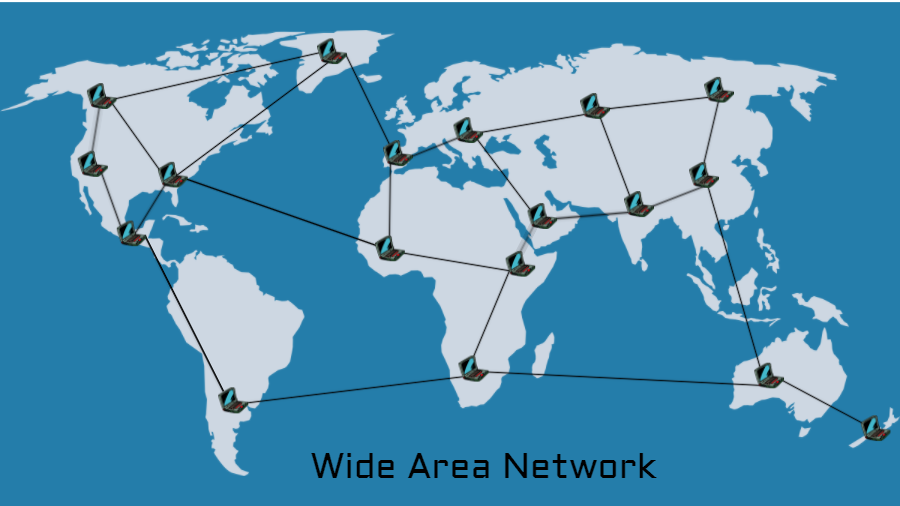
\includegraphics[scale=0.3]{WAN}
\end{center}
\centerline{Hình 2 : Mô phỏng hệ thống thông tin toàn cầu (internet).}
\changefontsizes{12pt}
\centerline{Nguồn: https://itsuksesindo.wordpress.com/}

\bigskip
\changefontsizes{14pt}
\setlength{\parindent}{0.2cm}
\textbf{III - Phân loại mạng máy tính}

\changefontsizes{13pt}
\bigskip
\setlength{\parindent}{0.2cm}
\textbf{\textit{LAN}} (local area network): hay còn gọi là "mạng cục bộ", là mạng tư nhân trong một toà nhà, một khu vực (trường học, cơ quan,...) khoảng vài km. Chúng nối các máy chủ và các máy trạm trong khu vực để chia sẻ tài nguyên và trao đổi thông tin.

\smallskip
\setlength{\parindent}{0.2cm}
\textbf{\textit{MAN}} (metropolitan area network): hay còn gọi là "mạng đô thị", là mạng có quy mô lớn hơn LAN, phạm vi vài km. Nó có thể là một nhóm bao gồm các văn phòng gần nhau trong thành phố thuộc mạng công cộng hoặc tư nhân.

\smallskip
\setlength{\parindent}{0.2cm}
\textbf{\textit{WAN}} (wide area network): hay còn gọi là "mạng diện rộng", dùng trong vùng địa lý lớn có phạm vi từ vài trăm cho đến vài ngàn km. Chúng là một tập hợp các máy nhằm thường được gọi là host hay end system. Các máy chính được nối nhau bởi các mạng con (subnet). Nhiệm vụ của mạng con là truyền nhận các thông điệp từ máy này sang máy khác.

\begin{center}
     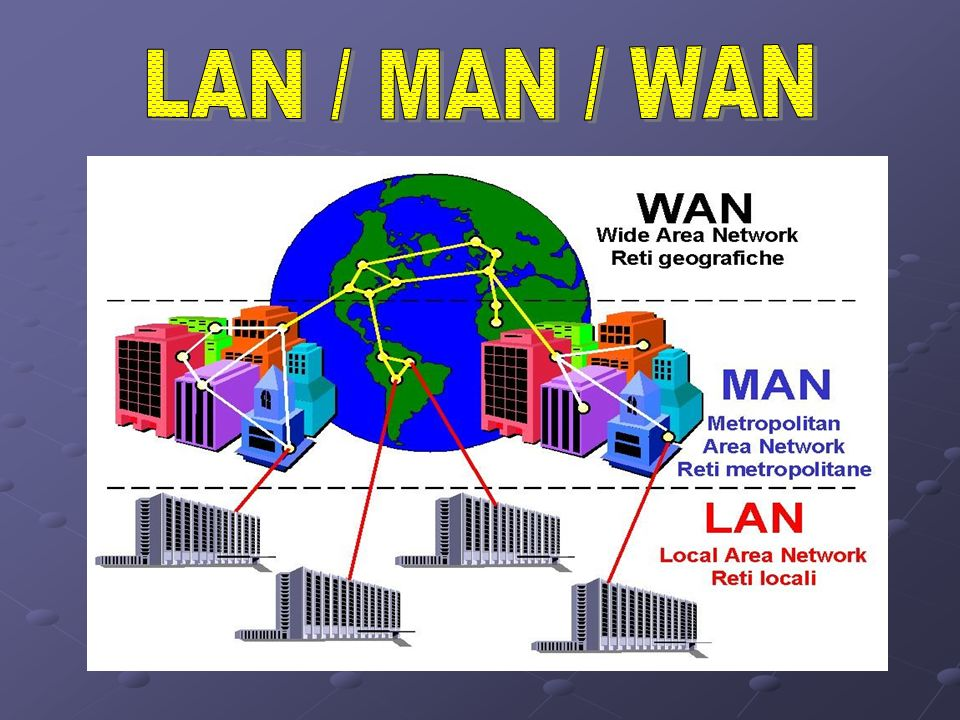
\includegraphics[scale=0.35]{lan_man_wan}
\end{center}
\centerline{Hình 3 : Minh họa LAN, MAN và WAN}
\changefontsizes{12pt}
\centerline{Nguồn: https://es.slideshare.net/NormaBezniuk}


\bigskip
\changefontsizes{14pt}
\setlength{\parindent}{0.2cm}
\textbf{IV - Các cấu trúc liên kết mạng máy tính}

\changefontsizes{13pt}
\bigskip
\setlength{\parindent}{0.2cm}
\textbf{\textit{Mạng hình sao (Star Network)}} Tất cả các trạm kết nối với một thiết bị trung tâm có nhiệm vụ chuyển tín hiệu từ các trạm gửi đến trạm đích. Tùy theo nhu cầu mà thiết bị trung tâm có thể là hub, switch, router, host hay end system.

\smallskip
\setlength{\parindent}{1cm}
Ưu điểm: đơn giản, dễ cấu hình, dễ kiểm soát và khắc phục sự cố, tận dụng được tối đa tốc độ truyền của đường truyền vật lý.

Khuyết điểm: độ dài đường truyền bị hạn chế.


\begin{center}
     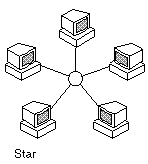
\includegraphics[scale=1]{star}
\end{center}
\centerline{Hình 4 : Minh họa mạng hình sao.}
\changefontsizes{12pt}
\centerline{Nguồn: https://www.webopedia.com/}

\changefontsizes{13pt}
\bigskip
\setlength{\parindent}{0.2cm}
\textbf{\textit{Mạng tuyến tính (Bus Network)}} Tất cả các trạm dùng chung một đường truyền. Đường truyền chính được giới hạn hai đầu bằng hai đầu nối đặc biệt gọi là điểm đầu cuối. 

\smallskip
\setlength{\parindent}{1cm}
Ưu điểm: dễ thiết kế và có chi phí thấp.

Khuyết điểm: tính ổn định kém.


\begin{center}
     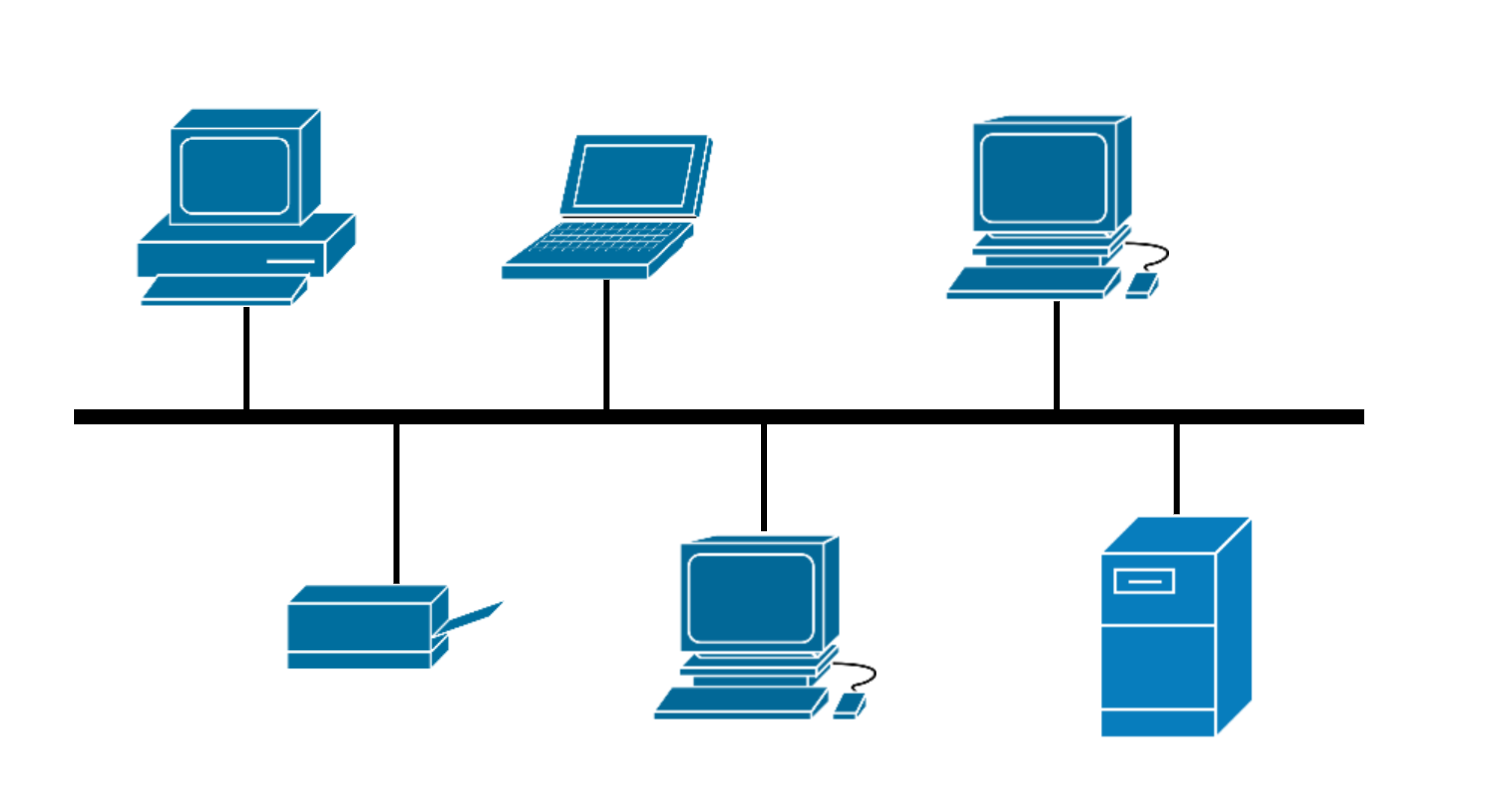
\includegraphics[scale=0.375]{bus}
\end{center}
\centerline{Hình 5 : Minh họa mạng tuyến tính.}
\changefontsizes{12pt}
\centerline{Nguồn: http://khoshamoz.ir/}

\bigskip
\changefontsizes{13pt}
\setlength{\parindent}{0.2cm}
\textbf{\textit{Mạng hình vòng (Ring Network)}} Mỗi trạm trên cấu trúc này chỉ kết nối tới một trạm kế và được một trạm khác kết nối tới tạo thành một mạch mạng hình vòng. Tín hiệu được truyền đi theo một chiều duy nhất.

\smallskip
\setlength{\parindent}{1cm}
Ưu điểm: đơn giản, dễ cấu hình, dễ kiểm soát và khắc phục sự cố, tận dụng được tối đa tốc độ truyền của đường truyền vật lý.

Khuyết điểm: dễ hỏng, khó thêm bớt trạm, giao thức truy nhập mạng phức tạp.



\begin{center}
     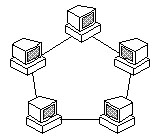
\includegraphics[scale=0.9]{ring}
\end{center}
\centerline{Hình 6 : Minh họa mạng hình vòng.}
\changefontsizes{12pt}
\centerline{Nguồn: https://www.webopedia.com/}

\changefontsizes{13pt}
\bigskip
\setlength{\parindent}{0.2cm}
\textbf{\textit{Mạng kết hợp (Mesh Network)}}

Kết hợp hình sao và tuyến tính (Star Bus Network): Cấu trúc này có bộ phận tách tín hiệu giữ vai trò là thiết bị trung tâm. Đem lại sự dễ dàng trong việc bố trí và có tương thích cao.

\begin{center}
     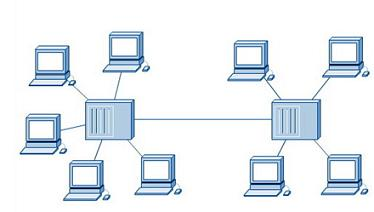
\includegraphics[scale=0.7]{starbus}
\end{center}
\centerline{Hình 7 : Minh họa mạng kết hợp hình sao và tuyến tính.}
\changefontsizes{12pt}
\centerline{Nguồn: http://thesis.binus.ac.id}


\bigskip
\changefontsizes{13pt}
\setlength{\parindent}{0.2cm}
Kết hợp hình sao và vòng (Star Ring Network): mỗi trạm làm việc được nối với HUB – là cầu nối giữa các trạm làm việc và để tǎng khoảng cách khi cần thiết.



\begin{center}
     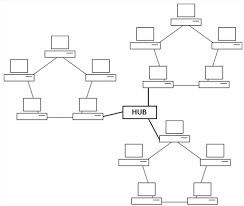
\includegraphics[scale=0.8]{starring}
\end{center}
\centerline{Hình 8 : Minh họa mạng kết hợp hình sao và vòng.}
\changefontsizes{12pt}
\centerline{Nguồn: https://www.thedailyprogrammer.com/}

\bigskip
\changefontsizes{14pt}
\setlength{\parindent}{0.2cm}
\textbf{V - Một số thiết bị mạng cơ bản}

\changefontsizes{13pt}
\bigskip
\setlength{\parindent}{0.2cm}
\textbf{\textit{Thiết bị truyền dẫn}}:

\smallskip
Cáp xoắn đôi (Twisted pair cable): gồm nhiều cặp dây đồng xoắn lại với nhau nhằm chống phát xạ nhiễu điện từ, có 2 loại: có và không có vỏ bọc chống nhiễu. Được sử dụng rộng rãi trong mạng LAN.

\smallskip
Cáp đồng trục (Coaxial Cable): là loại cáp điện với một lõi dẫn điện được bọc lại bởi một lớp điện môi không dẫn điện, chung quanh quấn thêm một lớp bện kim loại, ngoài cùng lại có vỏ bọc cách điện. Thường dùng làm đường truyền cho tín hiệu vô tuyến.

\smallskip
Cáp sợi quang (Fiber optic cable): là một loại cáp viễn thông làm bằng thủy tinh hoặc nhựa. Có bằng đường kính của một sợi tóc dài, mỏng và trong suốt được sắp xếp thành bó, sử dụng ánh sáng để truyền tín hiệu.


\begin{center}
     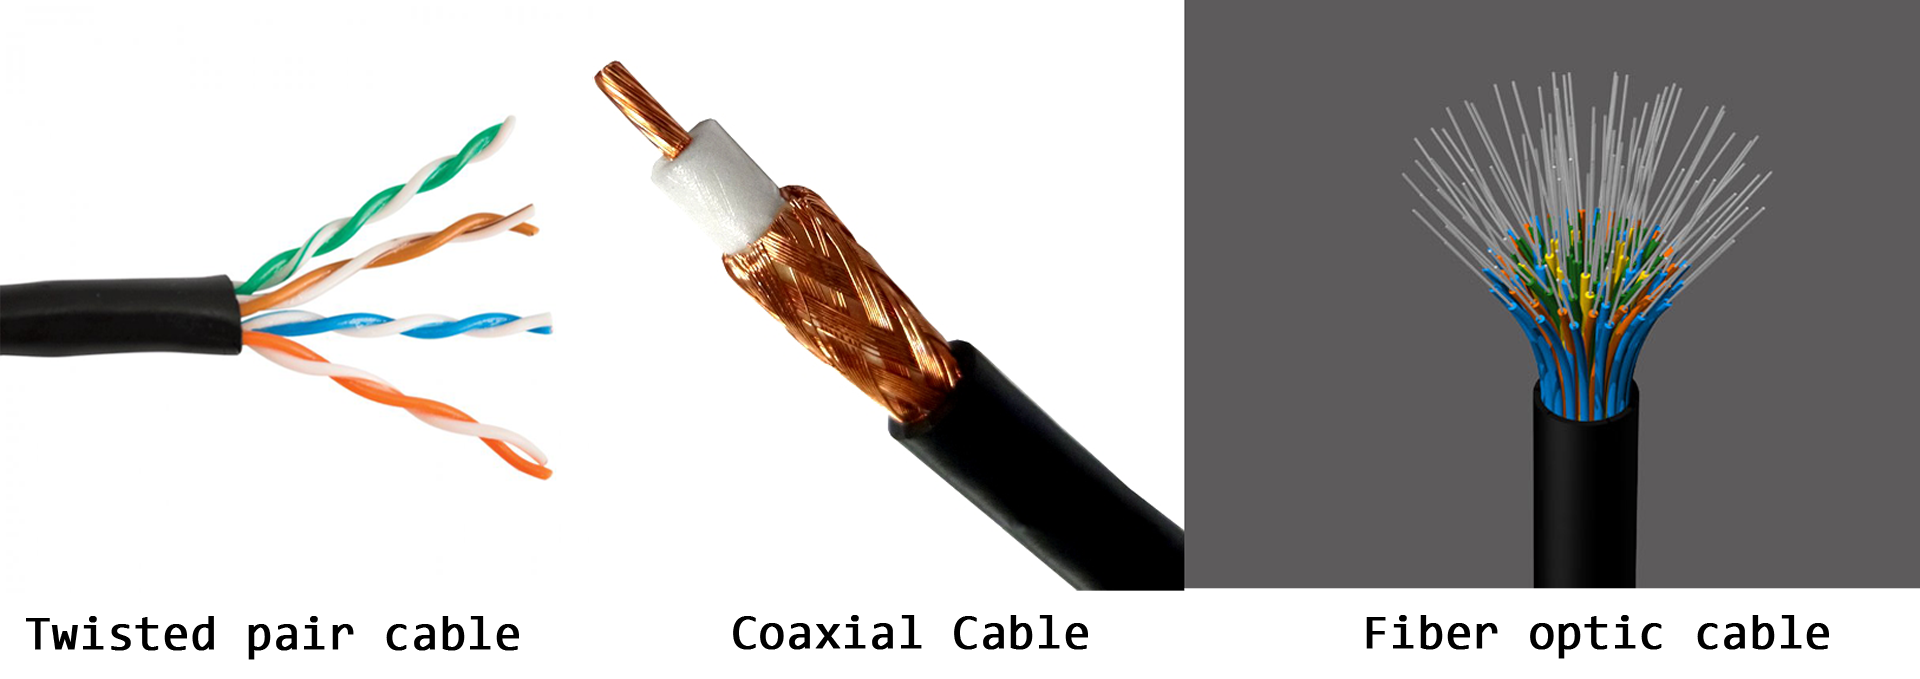
\includegraphics[scale=0.23]{cap}
\end{center}
\centerline{Hình 9 : Cáp xoắn đôi, Cáp đồng trục và Cáp sợi quang.}
\changefontsizes{12pt}
\centerline{Nguồn: https://fcit.usf.edu}
\changefontsizes{13pt}

\bigskip
\setlength{\parindent}{0.2cm}
\textbf{\textit{Thiết bị kết nối}}:

\smallskip
Repeater: là một bộ khuếch đại tín hiệu giữa hai cổng của hai phân đoạn mạng.

\begin{center}
     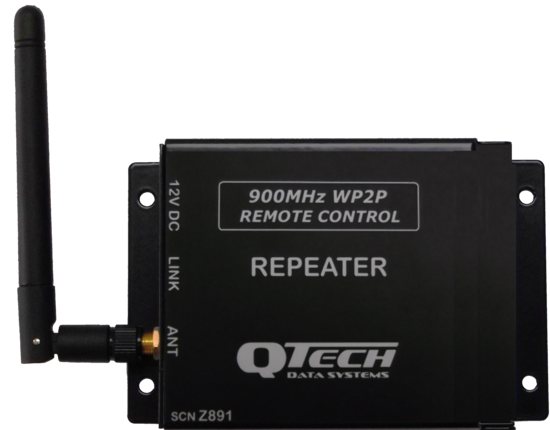
\includegraphics[scale=0.3]{repeater}
\end{center}
\centerline{Hình 10 : Một repeater.}
\changefontsizes{12pt}
\centerline{Nguồn: https://www.qtech.co.nz/}
\changefontsizes{13pt}

\bigskip
Router: là bộ định tuyến dùng để nối kết các thiết bị mạng vào trong cùng một mạng tương tác.


\begin{center}
     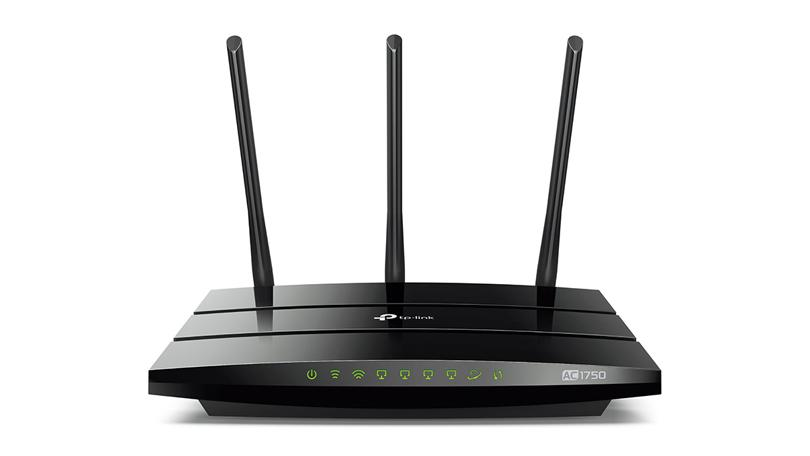
\includegraphics[scale=0.3]{router}
\end{center}
\centerline{Hình 11 : Một router.}
\changefontsizes{12pt}
\centerline{Nguồn: https://lifehacker.com/}
\changefontsizes{13pt}
\bigskip

Switch: là một thiết bị dùng để kết nối các thiết bị mạng với nhau theo mô hình mạng hình sao.

\begin{center}
     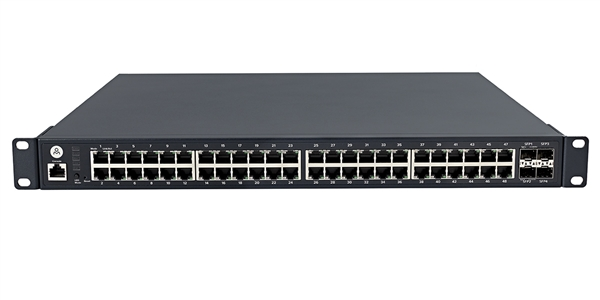
\includegraphics[scale=0.5]{switch}
\end{center}
\centerline{Hình 12 : Một switch.}
\changefontsizes{12pt}
\centerline{Nguồn: https://www.invictuswireless.com/}
\changefontsizes{13pt}
\bigskip


Hub: là thiết bị cho phép nhiều thiết bị mạng kết nối tập trung với nhau tại một điểm đồng thời khuếch đại tín hiệu giữa các phân đoạn mạng.

\begin{center}
     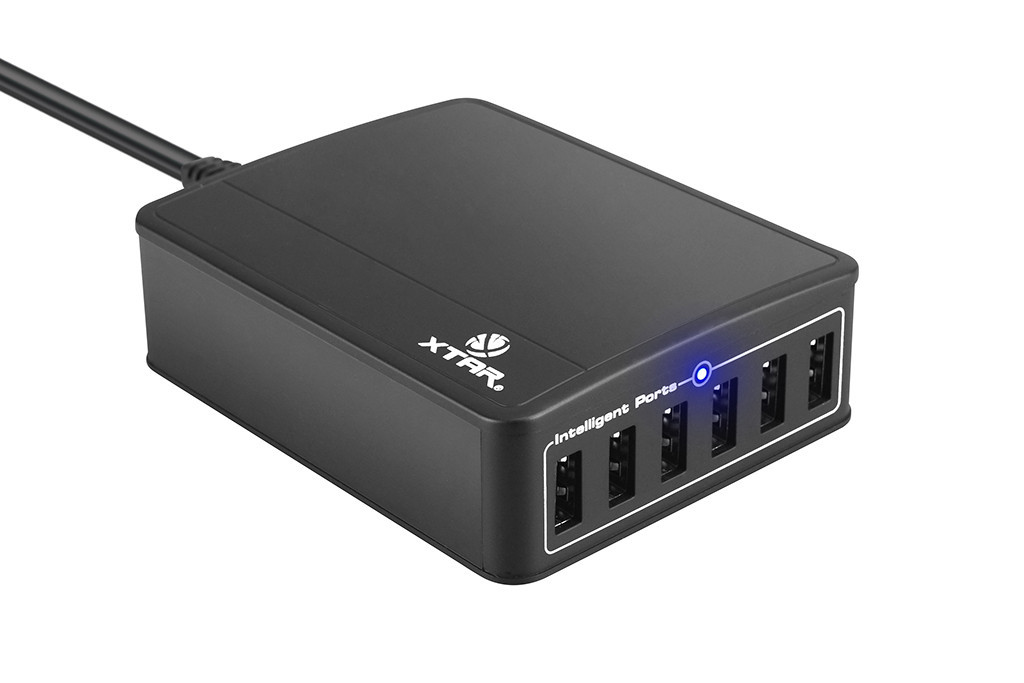
\includegraphics[scale=0.2]{hub}
\end{center}
\centerline{Hình 13 : Một hub.}
\changefontsizes{12pt}
\centerline{Nguồn: https://ru.nkon.nl/}
\changefontsizes{13pt}
\bigskip

\newpage
Bridge: là thiết bị cho phép nối kết hai nhánh mạng, có chức năng chuyển các gói tin một cách có chọn lọc. 



\begin{center}
     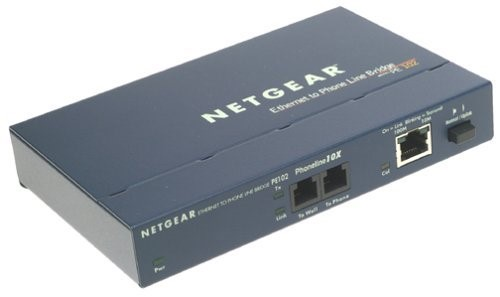
\includegraphics[scale=0.45]{bridge}
\end{center}
\centerline{Hình 14 : Một bridge.}
\changefontsizes{12pt}
\centerline{Nguồn: https://skilldevelopmentglobal.blogspot.com/}
\changefontsizes{13pt}
\bigskip


Gateway: là thiết bị trung gian dùng để nối kết những mạng khác nhau cả về kiến trúc lẫn môi trường mạng.

\begin{center}
     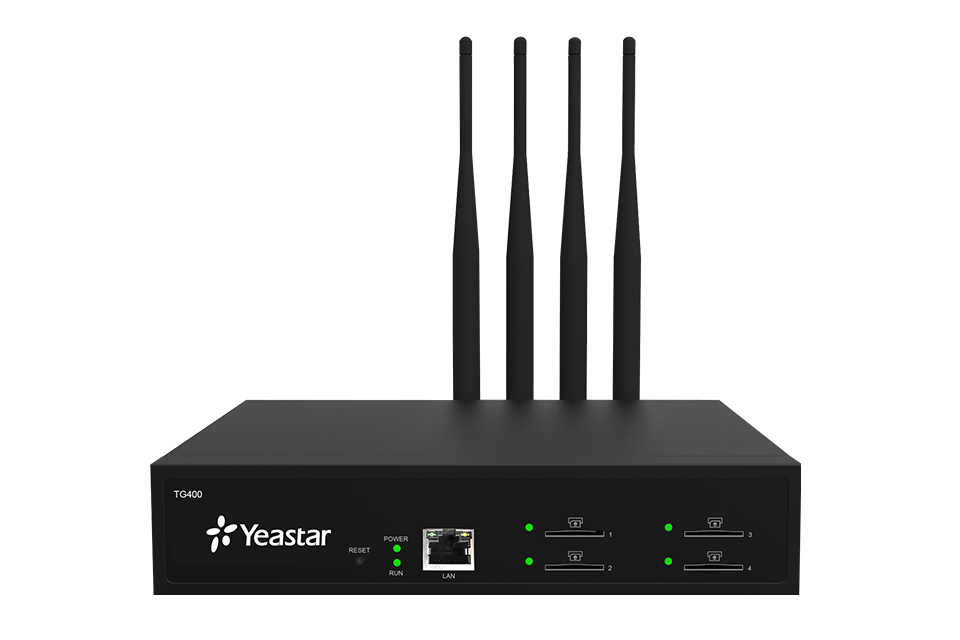
\includegraphics[scale=0.3]{gateway}
\end{center}
\centerline{Hình 15 : Một gateway.}
\changefontsizes{12pt}
\centerline{Nguồn: https://www.nexhi.com}
\changefontsizes{13pt}
\bigskip


%Page 14
\newpage
\changefontsizes{16pt}
\centerline{\textbf{PHẦN 2 : TIẾN HÀNH XÂY DỰNG VÀ CẤU HÌNH}}
\centerline{\textbf{HỆ THỐNG MẠNG}}

\bigskip
\changefontsizes{14pt}
\textbf{1.	Yêu cầu đề bài.}
\changefontsizes{13pt}

\bigskip
Xây dựng mạng máy tính cho tòa nhà C trường ĐH Tôn Đức Thắng, gồm các thiết bị đầu cuối DHCP, Server DNS, Server Web và Mail Server.

\bigskip
\changefontsizes{14pt}
\textbf{2.	Phân tích sơ đồ mạng.}
\changefontsizes{13pt}

\bigskip
Tòa nhà C bao gồm 1 trệt và 6 lầu. Mỗi tầng sẽ được lắp đặt một Router, các phòng sẽ thiết lập kết nối vào các Switch. Việc sử dụng kết nối thông qua những Switch dùng để cài đặt mạng VLAN cho tòa nhà C, tiến hành lắp đặt 5 Server lần lượt là: DHCP Server, Web Server, Mail Server, FTP Server và DNS Server. 

\bigskip
\changefontsizes{14pt}
\textbf{3.	Mô hình mạng:}
\changefontsizes{13pt}
\bigskip

\begin{center}
     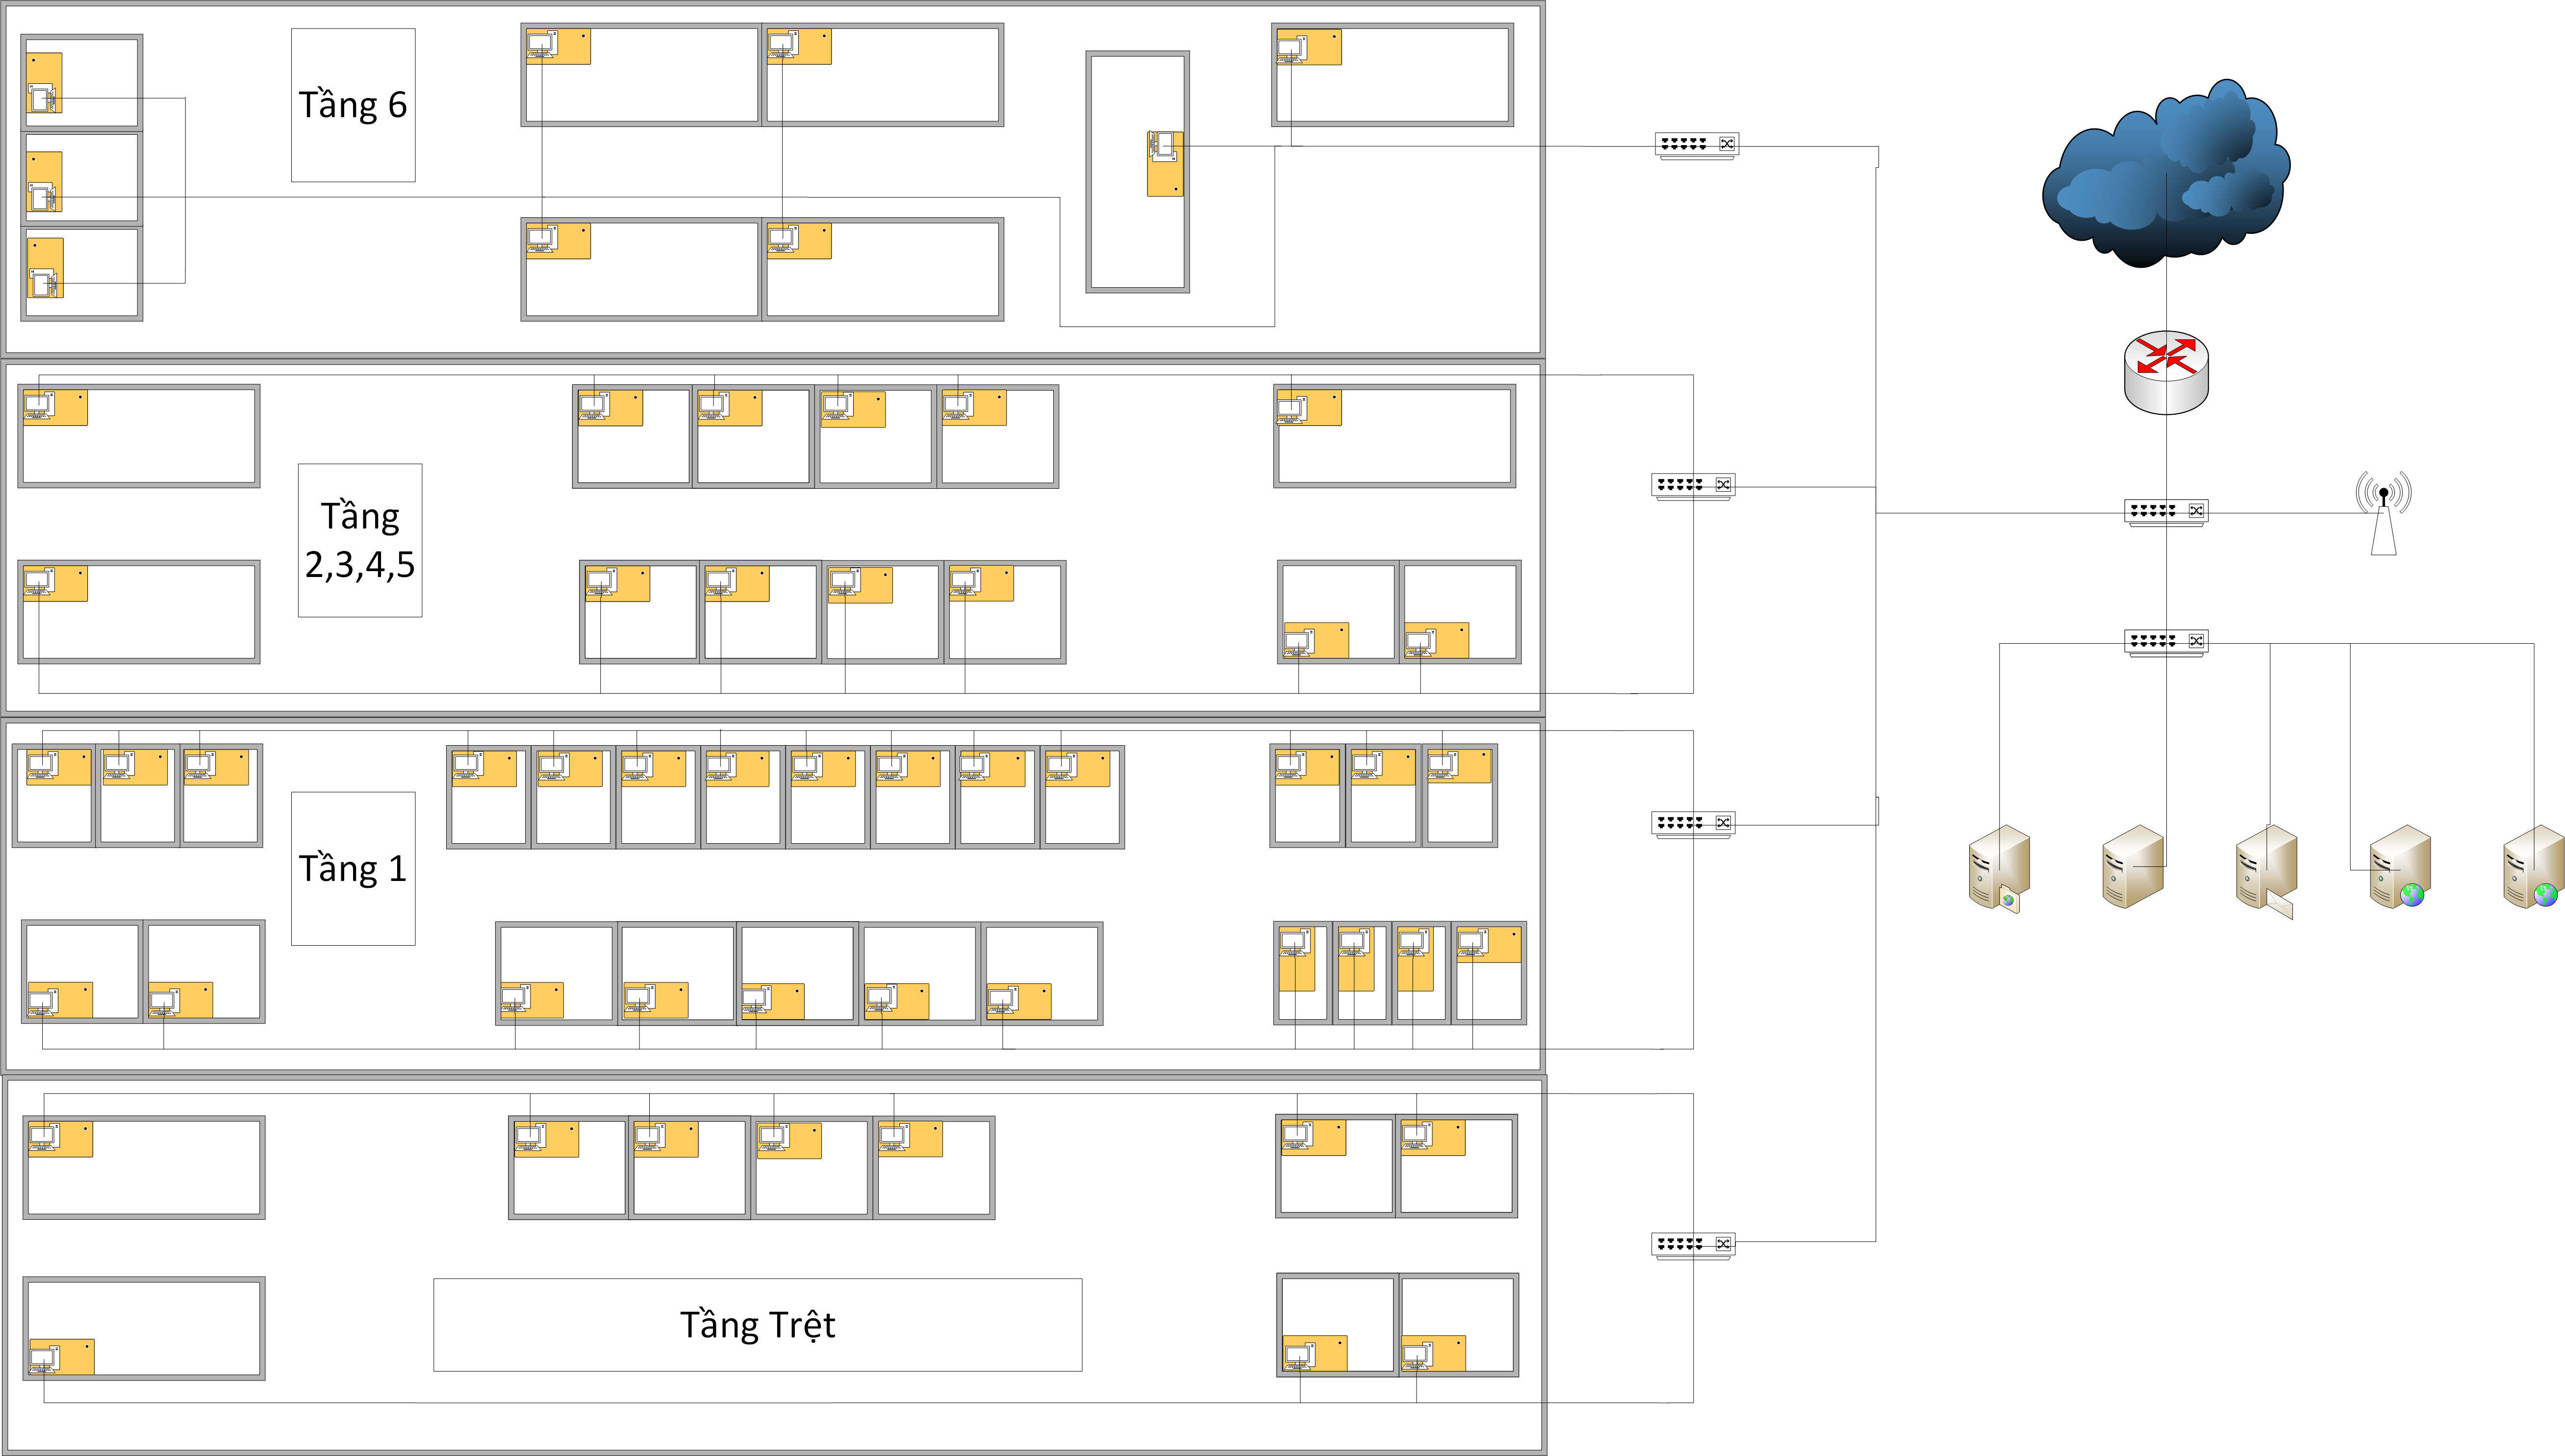
\includegraphics[scale=0.0825]{logic}
\end{center}
\centerline{Hình 16 : Sơ đồ mạng (vật lí) của tòa nhà C.}
\bigskip

\changefontsizes{14pt}
\textbf{4.	Các thiết bị mạng:}
\changefontsizes{12pt}
\smallskip

\begin{tabular}{|m{1.8cm}|m{7.6cm}|m{1cm}|m{3.2cm}|}
    \hline
    Loại thiết bị & Tên sản phẩm & Số lượng & Giá tiền\\
	\hline
	Switch & Switch TP-Link TL-SF1024D 24 port & 7 & 760.000 vnd\\
	\hline	
	Core Switch & Switch Volktek Men-3410 & 2 & 2.980.000 vnd\\
	\hline
	Router & Draytek Vigor 3220 & 1 & 8.790.000 vnd\\
	\hline
	Wireless Router & Router Wifi ASUS RT-AC68U & 1 & 4.659.000 vnd\\
	\hline
	Server & Dell PowerEdge T30 E3 1225v5–70093749 & 5 & 17.990.000 vnd\\
	\hline
	Dây cáp & Bộ cáp mạng APTEK UTP CAT.6 305m & 1 & 1.190.000 vnd\\
	\hline
	\multicolumn{3}{|c|}{Tổng chi phí} & 115.869.000 vnd\\
	\hline
\end{tabular}

\smallskip
\centerline{Bảng 1 : Giá tiền của các thiết bị mạng cần dùng.}

\bigskip
\changefontsizes{14pt}
\textbf{5.	Cấu hình trên Cisco Packet Tracer:}
\changefontsizes{13pt}
\bigskip

\begin{center}
     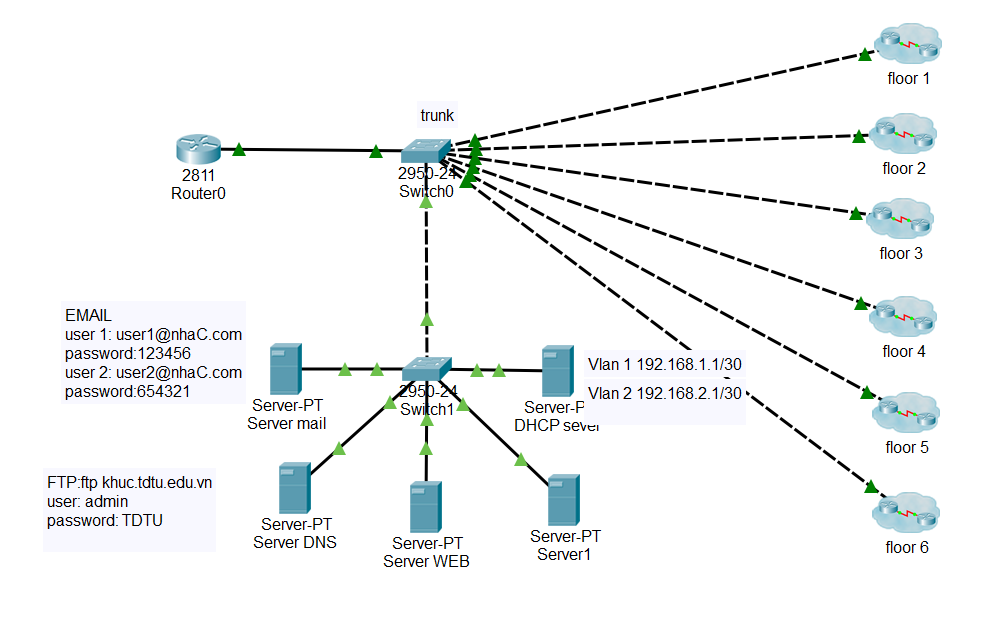
\includegraphics[scale=0.95]{cisco}
\end{center}
\centerline{Hình 17 : Sơ đồ mạng (luận lí) của tòa nhà C.}
\bigskip

\begin{center}
     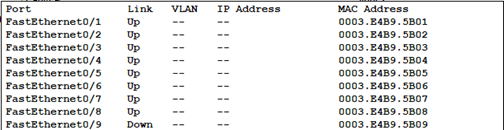
\includegraphics[scale=0.8]{im1}
\end{center}
\centerline{Hình 18 : Vlan trunking của switch core.}
\bigskip

\begin{center}
     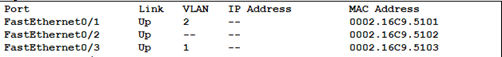
\includegraphics[scale=0.8]{im2}
\end{center}
\centerline{Hình 19 : Thiết kế vlan chung của các tầng, }
\centerline{với 2 vlan cho các phòng và 1 cổng trunking tới switch core.}
\bigskip

\begin{center}
     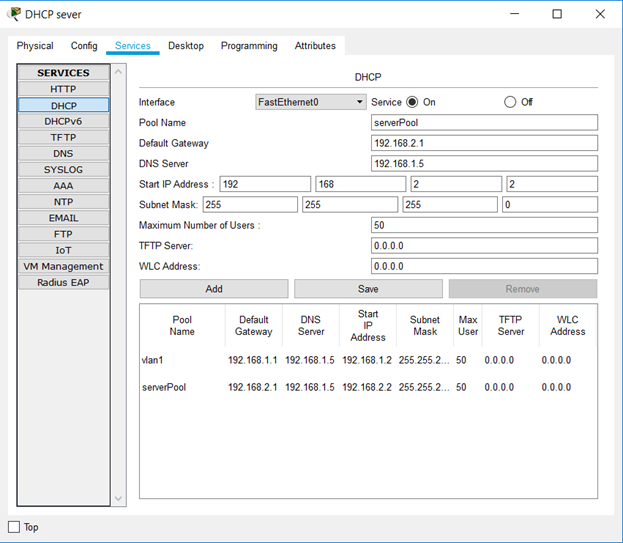
\includegraphics[scale=0.6]{im3}
\end{center}
\centerline{Hình 20 : DHCP cấp ip động cho 2 vlan 1 và 2 tương ứng với các máy của mỗi tầng.}
\bigskip


\newpage
\changefontsizes{16pt}
\centerline{\textbf{PHẦN 3 : THÔNG TIN CẤU HÌNH MẠNG}}
\changefontsizes{14pt}

\bigskip
\setlength{\parindent}{0.2cm}
\textbf{I - Thông tin kết nối port trong hệ thống}
\smallskip

\changefontsizes{12pt}

\begin{tabular}{|m{0.4cm}|m{2.15cm}|m{1.65cm}|m{2.2cm}|m{2.5cm}|m{1.6cm}|m{2cm}|}
    \hline
    No & Source to Destination Device & Source Interface&Destination Interface & Date Cable Lable & Protocol & Trunking /VLAN \\ 
    \hline
    1 & 2811(rt) to 2950T-24 (switch core) & Fa0/0 & Fa0/2 & RT-Fa0/0 --- SWCR-Fa0/2&Ethernet & Trunking \\ 
    \hline
    2 & 2950T-24 (switch core) to 2950T-24 (swf1) & Fa0/1 & Fa0/11 & SWCR-Fa0/1 --- SWF1-Fa0/1 & Ethernet & Trunking \\ 
    \hline
    3 & 2950T-24 (switch core) to 2950T-24 (swf2) & Fa0/4 & Fa0/2 & SWCR-Fa0/4 --- SWF2-Fa0/2 & Ethernet & Trunking \\
    \hline
    4 & 2950T-24 (switch core) to 2950T-24 (swf3) & Fa0/3 & Fa0/2 & SWCR-Fa0/3 --- SWF3-Fa0/2 & Ethernet & Trunking \\
    \hline
	5 & 2950T-24 (switch core) to 2950T-24 (swf4) & Fa0/5 & Fa0/2 & SWCR-Fa0/5 --- SWF4-Fa0/1 & Ethernet & Trunking \\
	\hline
	6 & 2950T-24 (switch core) to 2950T-24 (swf5) & Fa0/6 & Fa0/2 & SWCR-Fa0/6 --- SWF5-Fa0/2 & Ethernet & Trunking \\
	\hline
	7 & 2950T-24 (switch core) to 2950T-24 (swf6) & Fa0/7 & Fa0/2 & SWCR-Fa0/7 --- SWF6-Fa0/2 & Ethernet & Trunking \\
	\hline
\end{tabular}

\begin{tabular}{|m{0.4cm}|m{2.15cm}|m{1.65cm}|m{2.2cm}|m{2.5cm}|m{1.6cm}|m{2cm}|}
    \hline
	8 & 2950T-24 (switch sever) to DNS Server (DNS) & Fa0/2 & Fa0 & SWSV-Fa0/2 --- DNS-Fa0 & Ethernet & Trunking \\
	\hline
	9 & 2950T-24 (switch sever) to Mail Server (MAIL) & Fa0/1 & Fa0 & SWSV-Fa0/1 --- MAIL-Fa0 & Ethernet & Trunking \\
	\hline
	10 & 2950T-24 (switch sever) to Web Server (WEB) & Fa0/3 & Fa0 & SWSV-Fa0/3 --- WEB-Fa0 & Ethernet & Trunking \\
    \hline
	11 & 2950T-24 (switch core) to 2950T-24 (switch sever) & Fa0/8 & Fa0/4 & SWCR-Fa0/8 --- SWSV-Fa0/4 & Ethernet & Trunking \\
    \hline
    12 & 2950T-24 (swsv) to DHCP Server (DHCP) & Fa0/5 & Fa0 & SWCR-Fa0/5 --- DHCP-Fa0 & Ethernet & Trunking \\
    \hline    
\end{tabular}

\smallskip
\centerline{Bảng 2 : Thông tin kết nối port trong hệ thống}

\newpage
\changefontsizes{14pt}
\textbf{II - Thông tin vlan, interface vlan trong hệ thống}
\smallskip
\changefontsizes{12pt}

\begin{tabular}{|m{0.4cm}|m{2.4cm}|m{1.8cm}|m{3.4cm}|m{2.4cm}|m{2.3cm}|}
	\hline
	No & VLAN name & VLAN ID & VLAN description & \multicolumn{2}{|c|}{}\\
	\hline
	\multicolumn{4}{|c|}{HeadOffice Site} & Subnet & Default Gateway \\
	\hline
   	 1 & SeverVlan & trunk & Vlan for Server & 255.255.255.0 & 192.168.1.1 192.168.2.1 \\
	\hline
	 2 & UserVlan C1 & 1, 2 & Vlan for User & 255.255.255.0 & 192.168.1.1 192.168.2.1 \\
	 \hline
	 3 & UserVlan E2 & 1, 2 & Vlan for User & 255.255.255.0 & 192.168.1.1 192.168.2.1 \\
	 \hline
	 4 & UserVlan E3 & 1, 2 & Vlan for User & 255.255.255.0 & 192.168.1.1 192.168.2.1 \\
	 \hline
     5 & UserVlan E4 & 1, 2 & Vlan for User & 255.255.255.0 & 192.168.1.1 192.168.2.1 \\
     \hline
	 6 & UserVlan E5 & 1, 2 & Vlan for User & 255.255.255.0 & 192.168.1.1 192.168.2.1 \\
	 \hline
  	 7 & UserVlan E6 & 1, 2 & Vlan for User	& 255.255.255.0	& 192.168.1.1 192.168.2.1 \\
  	 \hline
\end{tabular}

\smallskip
\centerline{Bảng 3 : Thông tin vlan, interface vlan trong hệ thống}

\changefontsizes{14pt}
\newpage
\textbf{III - Thông tin IP Management}
\smallskip

\changefontsizes{12pt}
\begin{tabular}{|m{0.5cm}|m{3.6cm}|m{1.5cm}|m{1.1cm}|m{1.9cm}|m{2.3cm}|m{1.85cm}|}
	\hline
	No & Server & Interface & VLAN & IP Addess & Subnet & Gateway \\
    \hline
     A & UCS-FI & & & & &  \\
	\hline
	& Switch & & & & & \\
	\hline 
    1 & Swf1(Switch C1) & Mgmt & 1, 2 & DHCP & 255.255.255.0 & 192.168.1.1 192.168.2.1 \\
	\hline
	2 & Swf2(Switch C2) & Mgmt & 1, 2 & DHCP & 255.255.255.0 & 192.168.1.1 192.168.2.1 \\
	\hline	
	3 & Swf3(Switch C3) & Mgmt & 1, 2 & DHCP & 255.255.255.0 & 192.168.1.1 192.168.2.1 \\
	\hline	
	4 & Swf4(Switch C4) & Mgmt & 1, 2 & DHCP & 255.255.255.0 & 192.168.1.1 192.168.2.1 \\ 
	\hline	
	5 & Swf5(Switch C5) & Mgmt & 1, 2 & DHCP & 255.255.255.0 & 192.168.1.1 192.168.2.1 \\
	\hline	
	6 & Swf6(Switch C6) & Mgmt & 1, 2 & DHCP & 255.255.255.0 & 192.168.1.1 192.168.2.1 \\
	\hline	
	7 & Swsv(Switch Server) & Mgmt & Trunk & 192.168.1.5 To 192.168.1.8 & 255.255.255.0 & 192.168.1.1 192.168.2.1 \\
	\hline	
\end{tabular}


\smallskip
\centerline{Bảng 4 : Thông tin IP Management}


%Page ?? + 1
\newpage
\changefontsizes{16pt}
\centerline{\textbf{TÀI LIỆU THAM KHẢO}}

\vspace{1.2cm}
\changefontsizes{14pt}
\textbf{Tiếng Việt}

\changefontsizes{13pt}
\bigskip
\url{https://vi.wikipedia.org/wiki/Mạng_máy_tính}

\smallskip
\url{http://tbe.vn/kien-thuc-tong-hop/17689-lich-su-mang-may-tinh.html}

\smallskip
\url{https://learn.vtc.edu.vn/courses/lap-trinh-mang-can-ban/lectures}

\url{/3548605}

\smallskip
\url{https://vi.wikipedia.org/wiki/Cáp_đồng_trục}

\smallskip
\url{https://vi.wikipedia.org/wiki/Cáp_xoắn_đôi}

\smallskip
\url{https://vi.wikipedia.org/wiki/Cáp_quang}

\smallskip
\url{http://tuvancongnghe.net/kien-thuc-mang-may-tinh-co-ban-phan-1-t}

\url{ong-quan-ve-mang-may-tinh/}

\smallskip
\url{https://vi.wikipedia.org/wiki/Cấu_trúc_liên_kết_mạng}

\smallskip
\url{https://quantrimang.com/cap-mang-cat-6-la-gi-va-no-khac-cap-mang-}

\url{cat-5e-nhu-the-nao-143072}

\smallskip
\url{https://www.anphatpc.com.vn/}

\changefontsizes{14pt}
\bigskip
\textbf{Tiếng Anh}

\changefontsizes{13pt}
\bigskip
\url{https://en.wikipedia.org/wiki/Computer_network}


\smallskip
Shelly, Gary, et al. "Discovering Computers" 2003 Edition.

\smallskip
Kurose James F and Keith W. Ross : Computer Networking: A Top-Down Approach Featuring the Internet, Pearson Education 2005.



\end{document}